\documentclass[11pt,a4paper]{article}
\usepackage{graphicx}
\usepackage[french]{babel}
\usepackage[T1]{fontenc}
\usepackage[utf8]{inputenc}
\usepackage{color}
\usepackage{subcaption}
\usepackage{hyperref}

\begin{document}

\begin{figure}
        
\includegraphics[width=0.4\textwidth]{img/logoUniversite.png}
        \hfill
        
\includegraphics[width=0.4\textwidth]{img/logoInstitutInformatique.png}
\end{figure}

\title{
    \textcolor{blue}{Le Mans Université}\\
    Licence Informatique \textit{2ème année}\\
    Module 174UP02 Rapport de Projet\\
    \textbf{JurassicWar}
}
\author{Solène Orieux, Romane Saint-Léger, Hannah Sergent}
\date{\today}

\maketitle
\clearpage
\tableofcontents

\section{Introduction}
\subsection{Contexte}
\subsection{Énoncé du problème}
\subsection{Objectifs initiaux du projet}



\section{Conception}
\subsection{Principales règles du jeu}
\subsection{Foncionnalités prévues}



\section{Oraganisation du travail}
\subsection{Répartition des tâches}
\subsection{Planning prévisionnel}
\subsection{Outils de programmation utilisés}



\section{Developpement}
\subsection{Représentation du terrain par une matrice}

\subsection{Positionnement et mobilité des dinosaures}

\subsection{Système d’actions et outils à disposition du joueur}
\subsubsection{Mécanique des changements de tour}
\subsubsection{Infliger un coup mortel : bombe}
\subsubsection{Blesser un dinosaure : armes de tir}
\subsubsection{Autre méthode de déplacement : grapin}

\subsection{Interface graphique et utilisateur}
\subsubsection{Utilisation du module SDL}
\subsubsection{Création d’un menu principal}
\subsubsection{Faciliter l’utilisation du jeu pour l’utilisateur}



\section{Résultats et Conclusion}


\section{Bibliographie}
\newpage

\section{Annexes}
\subsection{Jeux de tests}
\subsection{Traces de débogage}
\subsubsection{Correction du système de collisions de la bombe}

Lors de la création des fonctions détectant un contact de la bombe avec le terrain, la mer et  les frontières de la fenêtre, un bug silencieux a été rencontré, necessitant l'usage de l'outil gdb pour identifier le dysfonctionnement. La situation est la suivante :
\begin{figure}[h]
	\centering
	\begin{subfigure}{0.45\textwidth}
	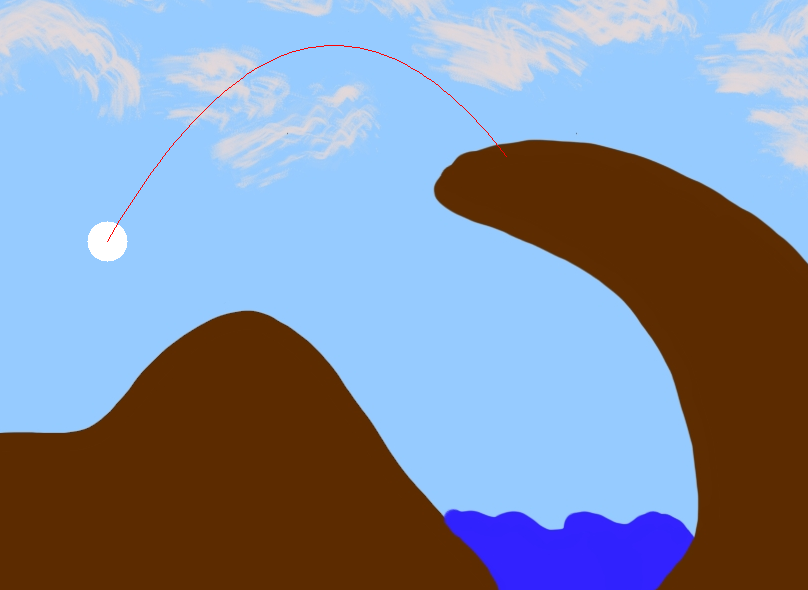
\includegraphics[height=3.5cm]{img/trajectoireCollisionBombe.png}
	\caption[trajectoire prevue]{Trajectoire prévue}
	\label{fig:trajectoireCollisionBombe}
	\end{subfigure}
	\hfill
	\begin{subfigure}{0.45\textwidth}
	
\includegraphics[height=3.5cm]{img/anomalieCollisionBombe.png}
	\caption[trajet effectue]{Trajet effectué}
	\label{fig:anomalieCollisionBombe}
	\end{subfigure}
	\caption[parcours incorrect de la bombe]{Parcours incorrect de la bombe}
	\label{fig:collisionBombe}
\end{figure}\\
La bombe interrompt sa trajectoire au milieu du terrain avant d'avoir heurté la terre. Il s'agit par conséquent d'identifier une erreur dans la fonction collisionTerrainBombe. Pour cela, les fichiers impliqués dans l'affichage et le système de collisions sont compilés avec l'option -g : 
gdb bombe\\
Initialiser l’affichage des variables :\\
(gdb) break testFonctionsRebonds.c :67\\
Simuler l’appui sur la touche b :\\
(gdb) break estFonctionsRebonds.c :92\\
Vérifier que le lancement de la bombe :\\
(gdb) break estFonctionsRebonds.c :98\\
Analyser les valeurs des variables à la suite d’une collision avec le terrain :\\
(gdb) break testFonctionsRebonds.c: 117\\
Provoquer un arrêt en cas de collision avec le terrain :\\
(gdb) break fonctionsRebonds.c:60 if ((matriceTerrain[bombe->coor.x][bombe->coor.y + bombe->rayon] == TERRE) || (matriceTerrain[bombe->coor.x][bombe->coor.y - bombe->rayon] == TERRE) || (matriceTerrain[bombe->coor.x + bombe->rayon][bombe->coor.y] == TERRE) || (matriceTerrain[bombe->coor.x - bombe->rayon][bombe->coor.y] == TERRE))\\
(gdb) run\\
(gdb) display bombeLancee\\
bombeLancee = 0\\
(gdb) display bombe.coor\\
bombe.coor = {x = 325, y = 350}\\
(gdb) continue\\
bombeLancee = 0\\
bombe.coor = {x = 325, y = 350}\\
(gdb) set etatClavier[5] = 1\\
(gdb) continue\\
Positionnement de la bombe afin que sa trajectoire rencontre le terrain\\
bombeLancee = 1\\
bombe.coor = {x = 325, y = 350}\\
(gdb) continue\\
Thread 1 "bombe" hit Breakpoint 5, rebondTerrainBombe (matriceTerrain=0x7fffffc85290, bombe=0x7fffffc85234) at fonctionsRebonds.c:60\\
60	    return ((matriceTerrain[bombe->coor.x][bombe->coor.y + bombe->rayon] == TERRE) || (matriceTerrain[bombe->coor.x][bombe->coor.y - bombe->rayon] == TERRE) || (matriceTerrain[bombe->coor.x + bombe->rayon][bombe->coor.y] == TERRE) || (matriceTerrain[bombe->coor.x - bombe->rayon][bombe->coor.y] == TERRE));\\
(gdb) continue\\
bombeLancee = 1\\
bombe.coor = {x = 592, y = 131}\\
(gdb) next\\
bombeLancee = 0\\
bombe.coor = {x = 592, y = 131}\\
(gdb) quit\\

\end{document}